Dense SLAM (Simultaneous Localisation and Mapping) has proven very effective for reconstructing moderately-sized scenes,
with much recent research driven by the availability of inexpensive, consumer-grade depth sensing equipment \cite{Newcombe2011,Niessner2013,Prisacariu2014}. 
However, accurate pose estimation in the presence of erroneous measurements and visual aliasing in the scene remains difficult to fully solve. Common approaches \cite{Besl1992,Levoy2001} exploit geometric/texture cues to estimate the pose of each frame, but tracking can drift -- or even fail completely -- without reliable features against which to track.
%Purely geometry based approaches may fail with a lack of descriptive geometry, as may texture based approaches with a lack of texture. 
%Common issues range from tracking drift, often caused by geometric and/or texture ambiguity, to complete tracking failure.
Loop closure events are another common source of tracking problems, with explicit handling often required to prevent errors in the model, exacerbating any existing tracking issues.
%In addition, many dense SLAM systems fail during loop closure events, with explicit handling often required. The error incurred during loop closure events can be detrimental to tracking quality in such systems.
These problems are only magnified when reconstructing objects: an object's surface will generally contain far fewer points than the full scene, and a lack of unambiguous points on the surface can lead to an increase in data association errors when attempting to recover the pose.

%Failure cases for such approaches are only exacerbated by having less data to track with/against, as is the case with the tracking of an object's pose w.r.t.\ the camera (the inverse of the camera tracking problem). In the case of tracking an object's motion w.r.t.\ the static scene, only the object surface points are available for tracking.

%As dense object reconstruction can be seen as a smaller-scale equivalent of the dense scene reconstruction problem, it too is prone to 
%tracking drift and loop closure issues, sometimes to a prohibitive level. As previously highlighted, the tracking of an object's pose w.r.t.\ the camera 
%is also affected by geometric or texture-based ambiguities, caused by a much more focused domain of the data available to the tracking algorithm. 
%Such failure cases may occur with the presence of ambiguous features, and a lack of unambiguous features on the object surface, causing data 
%association errors when attempting to recover pose.

%For example, when reconstructing an entire scene and assuming no masking, all of the data in the current and previous frames is available for tracking. When tracking solely an object this is not the case as attempting to track an objects movement w.r.t.\ static scene points and dynamic object points would cause a failure event.

In this paper, we introduce a novel approach to reconstruct accurate, globally-consistent object models, introducing a probabilistic rigid-object reconstruction 
framework based on depth features. The framework facilitates the correction of tracking drift by representing the object as a
collection of overlapping subsegments between which transformations may be inferred to maintain alignment, resulting in a consistent
overall model. By combining these transformed surfaces, we extract an implicitly deformed surface, optimised for via the probabilistic formulation 
that follows. We utilise a volumetric representation for each of these object subsegments, with each voxel in a given subsegment having additional appearance posterior 
information pertaining to the voxel's membership of the object. Over time, multiple volumes containing both surface and probabilistic appearance information are 
maintained and manipulated to yield a robust and temporally consistent model. Finally, we optimise for the optimum object segmentation within a CRF (Conditional Random Field) framework.

Recently, robust, globally-consistent, large scale scene reconstruction has been achieved by combining a multi-segment representation with loop closure detection and an online model correction algorithm \cite{Kahler2016}, demonstrating the efficacy of this approach for larger scenes.

\begin{figure}[!t]
	\centering
	\begin{tabular}{cc}
		%\fbox{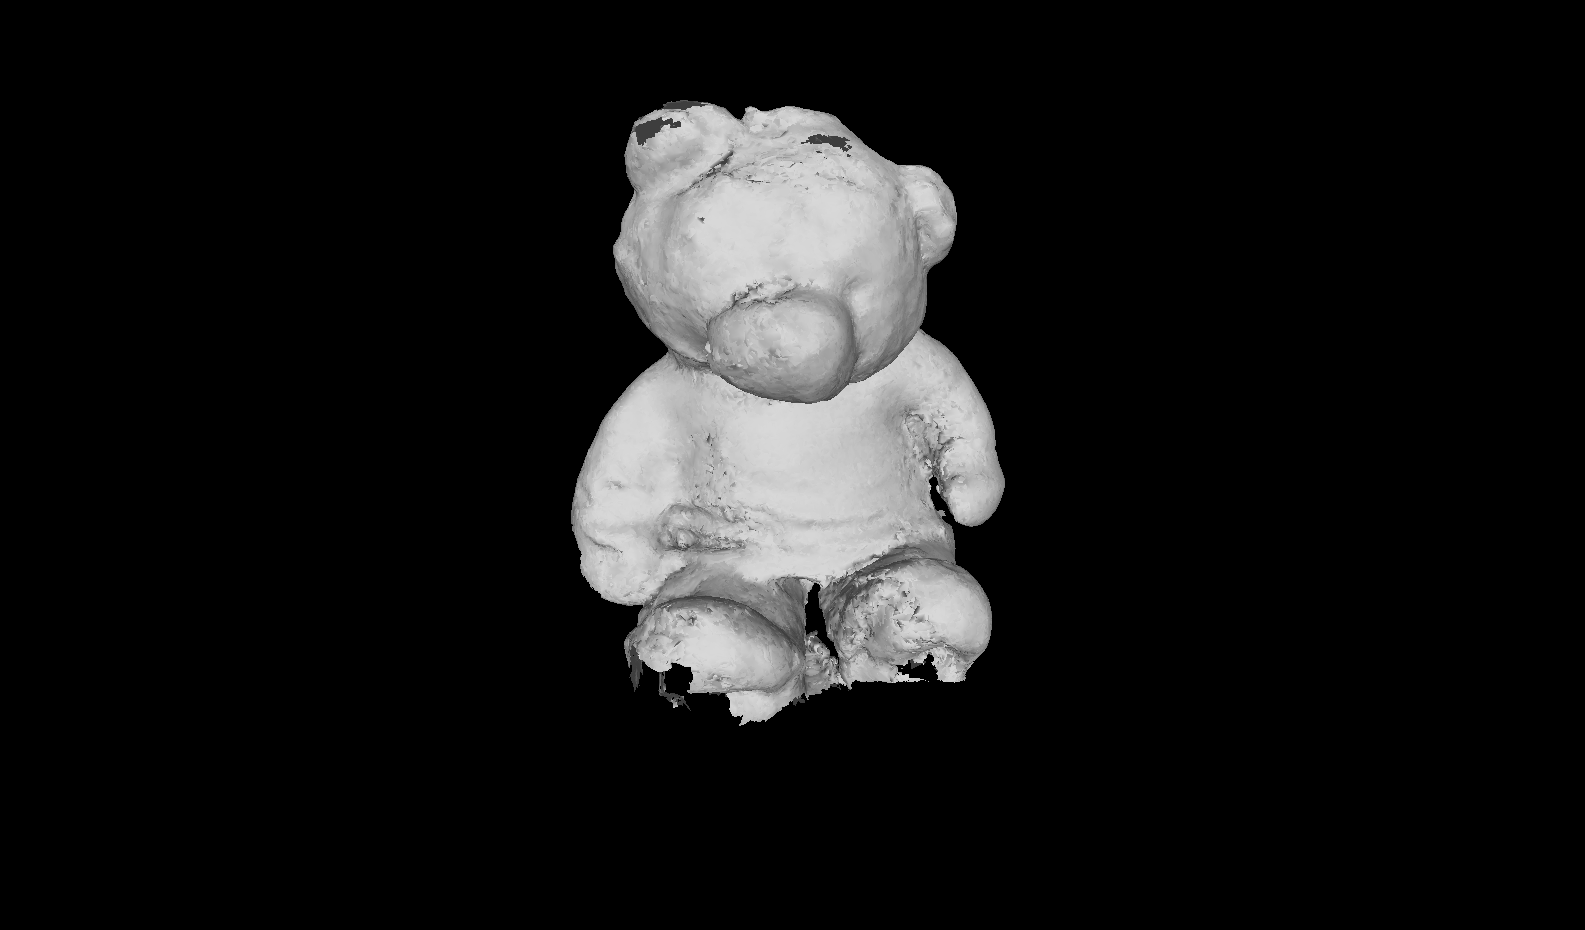
\includegraphics[width=3cm]{screenshots/untextured/bear00.png}}&
		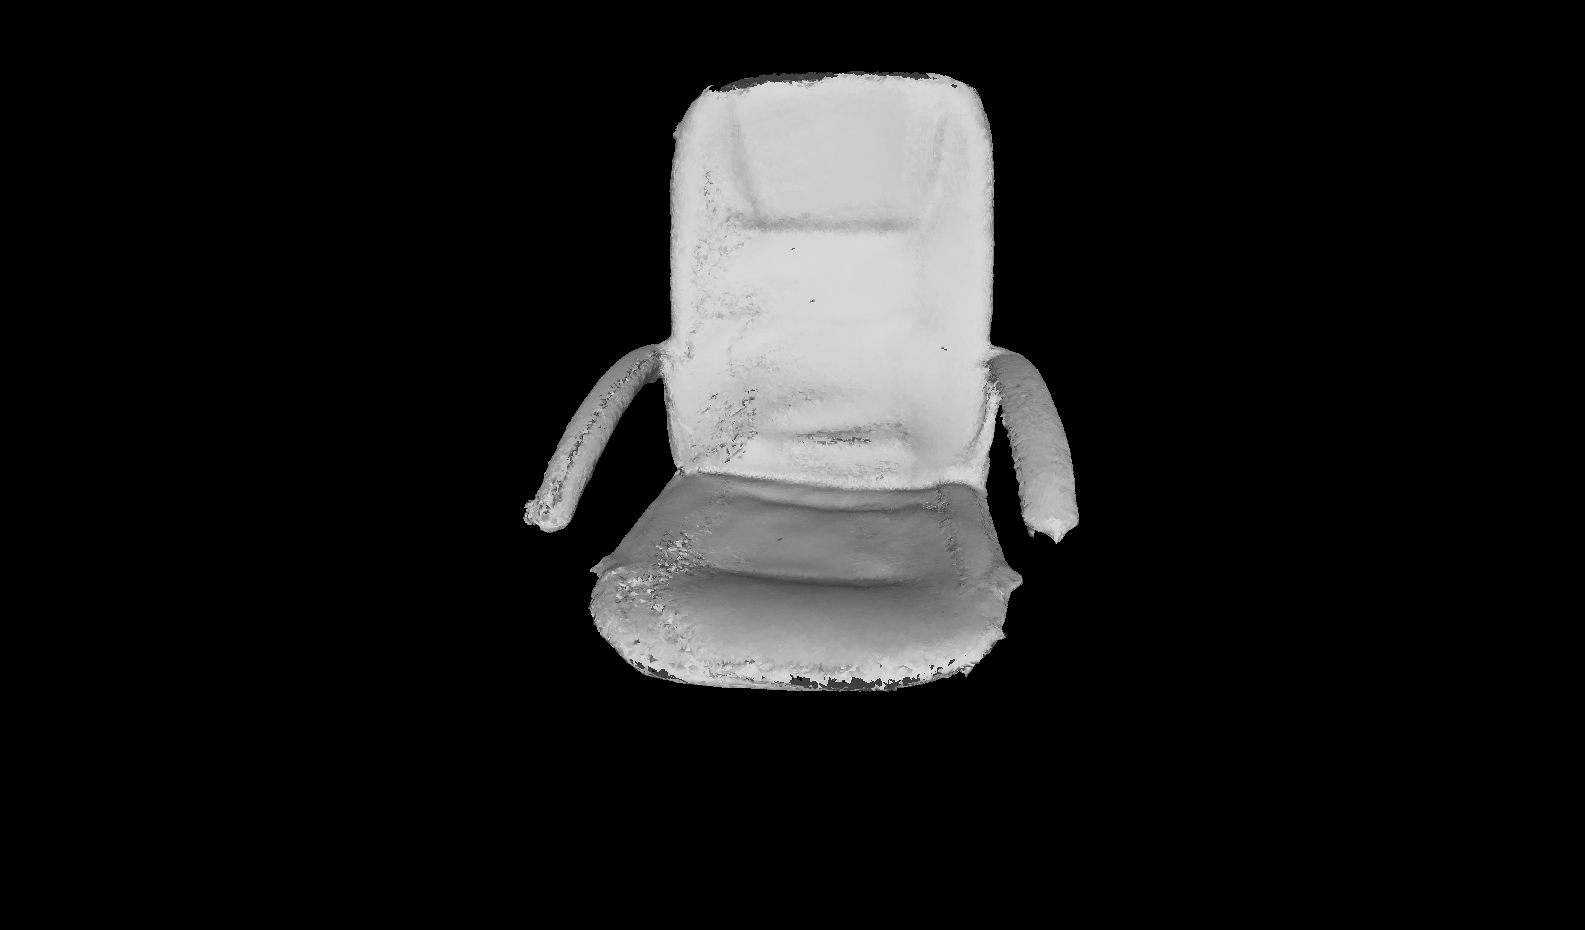
\includegraphics[width=3cm]{screenshots/untextured/chair00.png}&
		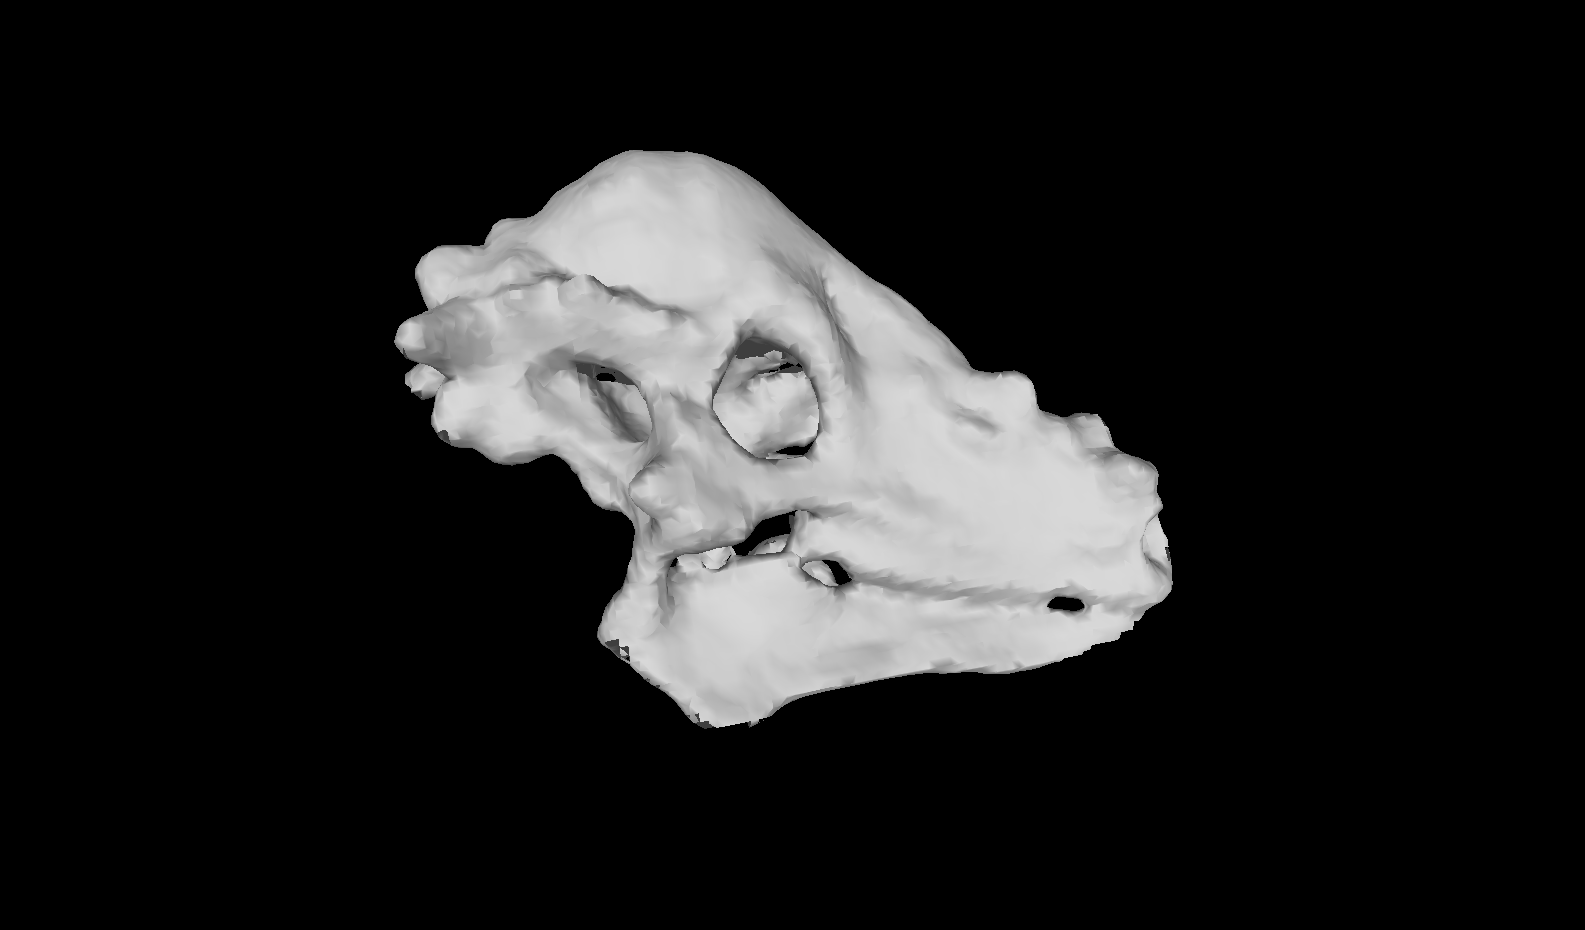
\includegraphics[width=3cm]{screenshots/untextured/dino00.png}
		%\fbox{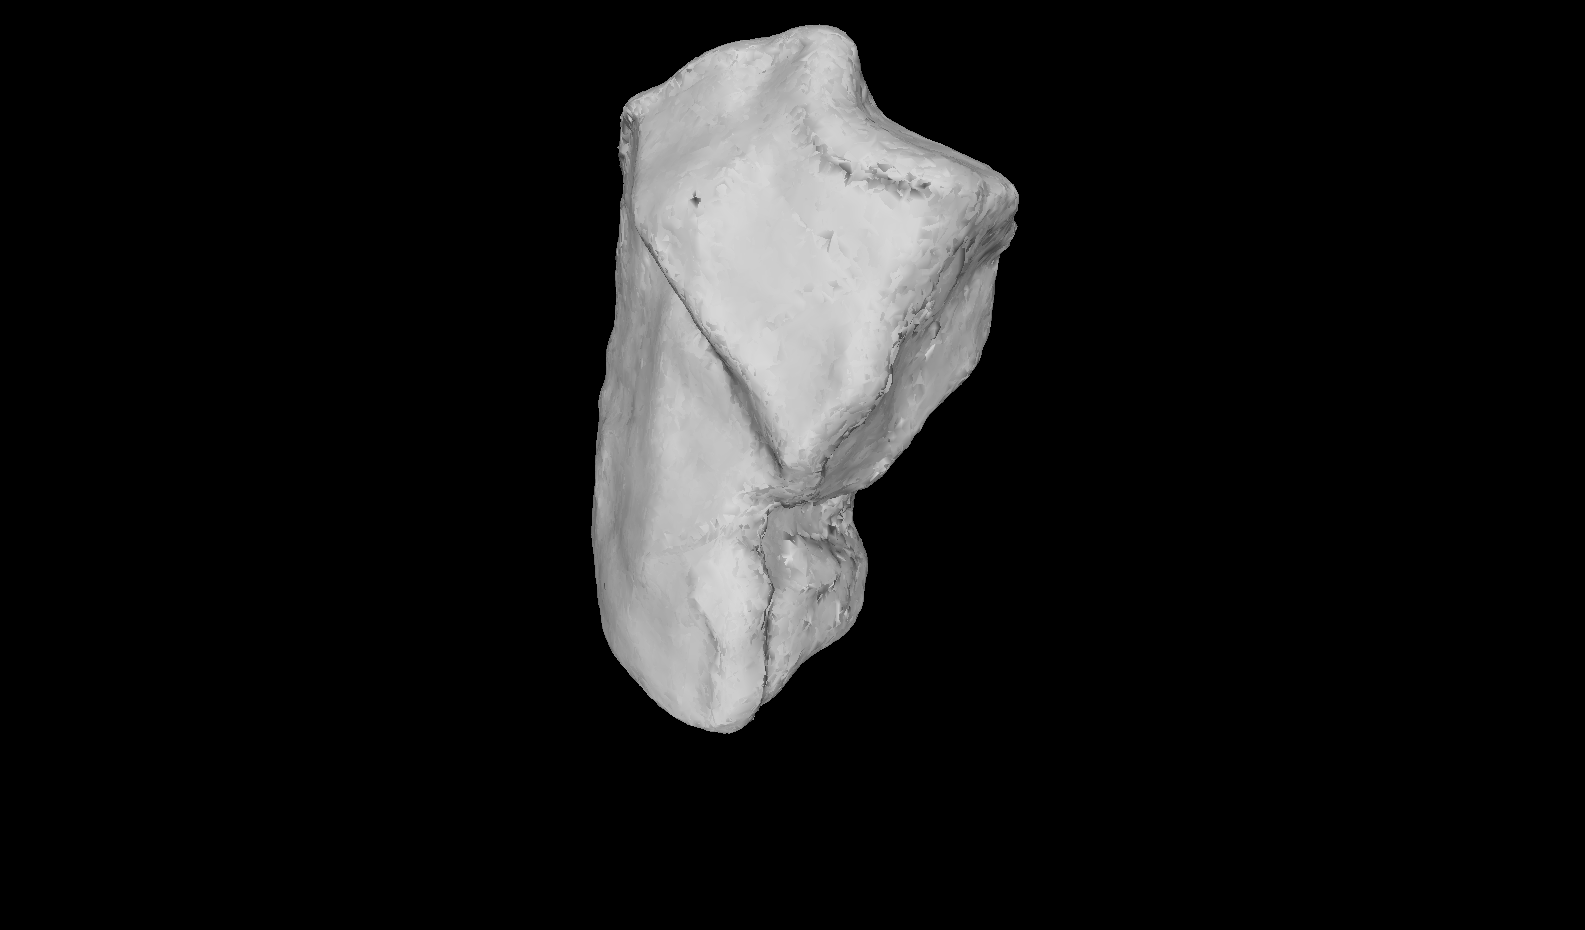
\includegraphics[width=3cm]{screenshots/untextured/rock00.png}}\\
	\end{tabular}
	\vspace{-3mm}
	\caption{
		Chair and Dinosaur Head reconstructed with our system.
		%\textbf{(a)} Teddy,
		%\textbf{(b)} Chair,
		%\textbf{(c)} Dinosaur Dead,
		%\textbf{(d)} Museum Rock.
	}
	\label{fig:demo}
\end{figure}
%We demonstrate efficacy in object reconstruction by performing online transformations to the aforementioned subsegments to counteract inconsistencies caused by drift in the object pose tracking process.
We perform both quantitative and qualitative experiments to compare our approach to the state-of-the-art object reconstruction approach of Ren et al.\ \cite{Ren2013}, demonstrating compelling improvements in both pose estimation and model quality. In addition we demonstrate compelling results over the standard KinectFusion pipeline using an open implementation \cite{Prisacariu2014} as a benchmark.

%We perform quantitative and qualitative experiments and demonstrate efficacious pose estimation and reconstruction quality respectively. As a base for comparison, tracking quality is compared with a well established dense SLAM evaluation benchmark \cite{sturm12iros} and reconstruction quality with the object reconstruction system outlined in \cite{Ren2013}.